\documentclass[12pt,hidelinks]{article}
	\usepackage[explicit]{titlesec}
	\usepackage{titletoc}
	\usepackage{tocloft}
	\usepackage{charter}
	\usepackage[many]{tcolorbox}
	\usepackage{amsmath}
	\usepackage{graphicx}
	\usepackage{xcolor}
	\usepackage{tikz,lipsum,lmodern}
	\usetikzlibrary{calc}
	\usepackage[english]{babel}
	\usepackage{fancyhdr}
	\usepackage{mathrsfs}
	\usepackage{empheq}
	\usepackage{fourier}% change to lmodern if fourier is no available
	\usepackage{wrapfig}
	\usepackage{fancyref}
	\usepackage{hyperref}
	\usepackage{cleveref}
	\usepackage{listings}
	\usepackage{varwidth}
	\usepackage{longfbox}
	\usepackage{geometry}
	\usepackage{marginnote}
	\tcbuselibrary{theorems}
	\tcbuselibrary{breakable, skins}
	\tcbuselibrary{listings, documentation}
	\geometry{
		a4paper,
		left=33mm,
		right=33mm,
		top=20mm}
% ========= Path to images ============
%   - Direct the computer on the path 
% 	  to the folder containg the images
% =====================================
\graphicspath{{./img/}}
% ============= Macros ================
\newcommand{\fillin}{\underline{\hspace{.75in}}{\;}}
\newcommand{\solution}{\textcolor{mordantred19}{Solution:}}
\setlength{\parindent}{0pt}
\addto{\captionsenglish}{\renewcommand*{\contentsname}{Table of Contents}}
\linespread{1.2}
% ======== Footers & Headers ==========
\cfoot{\thepage}
\chead{}\rhead{}\lhead{}
% =====================================
\renewcommand{\thesection}{\arabic{section}}
\newcommand\sectionnumfont{% font specification for the number
	\fontsize{380}{130}\color{myblueii}\selectfont}
\newcommand\sectionnamefont{% font specification for the name "PART"
	\normalfont\color{white}\scshape\small\bfseries }
% ============= Colors ================
% ----- Red -----
\definecolor{mordantred19}{rgb}{0.68, 0.05, 0.0}
% ----- Blue -----
\definecolor{st.patrick\'sblue}{rgb}{0.14, 0.16, 0.48}
\definecolor{teal}{rgb}{0.0, 0.5, 0.5}
\definecolor{beaublue}{rgb}{0.74, 0.83, 0.9}
\definecolor{mybluei}{RGB}{0,173,239}
\definecolor{myblueii}{RGB}{63,200,244}
\definecolor{myblueiii}{RGB}{199,234,253}
% ---- Yellow ----
\definecolor{blond}{rgb}{0.98, 0.94, 0.75}
\definecolor{cream}{rgb}{1.0, 0.99, 0.82}
% ----- Green ------
\definecolor{emerald}{rgb}{0.31, 0.78, 0.47}
\definecolor{darkspringgreen}{rgb}{0.09, 0.45, 0.27}
% ---- White -----
\definecolor{ghostwhite}{rgb}{0.97, 0.97, 1.0}
\definecolor{splashedwhite}{rgb}{1.0, 0.99, 1.0}
% ---- Grey -----
\definecolor{whitesmoke}{rgb}{0.96, 0.96, 0.96}
\definecolor{lightgray}{rgb}{0.92, 0.92, 0.92}
\definecolor{floralwhite}{rgb}{1.0, 0.98, 0.94}
% ========= Part Format ==========
\titleformat{\section}
{\normalfont\huge\filleft}
{}
{20pt}
{\begin{tikzpicture}[remember picture,overlay]
	\fill[myblueiii] 
	(current page.north west) rectangle ([yshift=-13cm]current page.north east);   
\node[
	fill=mybluei,
	text width=2\paperwidth,
	rounded corners=6cm,
	text depth=18cm,
	anchor=center,
	inner sep=0pt] at (current page.north east) (parttop)
	{\thepart};%
\node[
	anchor=south east,
	inner sep=0pt,
	outer sep=0pt] (partnum) at ([xshift=-20pt]parttop.south) 
	{\sectionnumfont\thesection};
\node[
	anchor=south,
	inner sep=0pt] (partname) at ([yshift=2pt]partnum.south)   
	{\sectionnamefont SECTION};
\node[
	anchor=north east,
	align=right,
	inner xsep=0pt] at ([yshift=-0.5cm]partname.east|-partnum.south) 
	{\parbox{.7\textwidth}{\raggedleft#1}};
\end{tikzpicture}%
}
% ========= Hyper Ref ===========
\hypersetup{
	colorlinks,
	linkcolor={red!50!black},
	citecolor={blue!50!black},
	urlcolor={blue!80!black}
}
% ========= Example Boxes =============
\tcbset{
	defstyle/.style={
		fonttitle=\bfseries\upshape, 
		fontupper=\slshape,
		arc=0mm, 
		beamer,
		colback=blue!5!white,
		colframe=blue!75!black},
	theostyle/.style={
		fonttitle=\bfseries\upshape, 
		fontupper=\slshape,
		colback=red!10!white,
		colframe=red!75!black},
	visualstyle/.style={
		height=6.5cm,
		breakable,
		enhanced,
		leftrule=0pt,
		rightrule=0pt,
		bottomrule=0pt,
		outer arc=0pt,
		arc=0pt,
		colframe=mordantred19,
		colback=lightgray,
		attach boxed title to top left,
		boxed title style={
			colback=mordantred19,
			outer arc=0pt,
			arc=0pt,
			top=3pt,
			bottom=3pt,
		},
		fonttitle=\sffamily,},
	discussionstyle/.style={
		height=6.5cm,
		breakable,
		enhanced,
		rightrule=0pt,
		toprule=0pt,
		outer arc=0pt,
		arc=0pt,
		colframe=mordantred19,
		colback=lightgray,
		attach boxed title to top left,
		boxed title style={
			colback=mordantred19,
			outer arc=0pt,
			arc=0pt,
			top=3pt,
			bottom=3pt,
		},
		fonttitle=\sffamily},
	mystyle/.style={
		height=6.5cm,
		breakable,
		enhanced,
		rightrule=0pt,
		leftrule=0pt,
		bottomrule=0pt,
		outer arc=0pt,
		arc=0pt,
		colframe=mordantred19,
		colback=lightgray,
		attach boxed title to top left,
		boxed title style={
			colback=mordantred19,
			outer arc=0pt,
			arc=0pt,
			top=3pt,
			bottom=3pt,
		},
		fonttitle=\sffamily},
	aastyle/.style={
			height=3.5cm,
			enhanced,
			colframe=teal,
			colback=lightgray,
			colbacktitle=floralwhite,
			fonttitle=\bfseries,
			coltitle=black,
		attach boxed title to top center={
	  		yshift=-0.25mm-\tcboxedtitleheight/2,
	   		yshifttext=2mm-\tcboxedtitleheight/2}, 
		boxed title style={boxrule=0.5mm,
			frame code={ \path[tcb fill frame] ([xshift=-4mm]frame.west)
				-- (frame.north west) -- (frame.north east) -- ([xshift=4mm]frame.east)
				-- (frame.south east) -- (frame.south west) -- cycle; },
			interior code={ 
				\path[tcb fill interior] ([xshift=-2mm]interior.west)
				-- (interior.north west) -- (interior.north east)
				-- ([xshift=2mm]interior.east) -- (interior.south east) -- (interior.south west)
				-- cycle;} }
				},
	examstyle/.style={
		height=9.5cm,
		breakable,
		enhanced,
		rightrule=0pt,
		leftrule=0pt,
		bottomrule=0pt,
		outer arc=0pt,
		arc=0pt,
		colframe=mordantred19,
		colback=lightgray,
		attach boxed title to top left,
		boxed title style={
			colback=mordantred19,
			outer arc=0pt,
			arc=0pt,
			top=3pt,
			bottom=3pt,
		},
		fonttitle=\sffamily},
	doc head command={
		interior style={
			fill,
			left color=yellow!20!white, 
			right color=white}},
	doc head environment={
		boxsep=4pt,
		arc=2pt,
		colback=yellow!30!white,
		},
	doclang/environment content=text
}
% ============= Boxes ================
\newtcolorbox[auto counter,number within=section]{example}[1][]{
	mystyle,
	title=Example~\thetcbcounter,
	overlay unbroken and first={
		\path
		let
		\p1=(title.north east),
		\p2=(frame.north east)
		in
		node[anchor=
			west,
			font=\sffamily,
			color=st.patrick\'sblue,
			text width=\x2-\x1] 
		at (title.east) {#1};
	}
}
\newtcolorbox[auto counter,number within=section]{longexample}[1][]{
	examstyle,
	title=Example~\thetcbcounter,
	overlay unbroken and first={
		\path
		let
		\p1=(title.north east),
		\p2=(frame.north east)
		in
		node[anchor=
		west,
		font=\sffamily,
		color=st.patrick\'sblue,
		text width=\x2-\x1] 
		at (title.east) {#1};
	}
}
\newtcolorbox[auto counter,number within=section]{example2}[1][]{
	aastyle,
	title=Example~\thetcbcounter,{}
}
\newtcolorbox[auto counter,number within=section]{discussion}[1][]{
	discussionstyle,
	title=Discussion~\thetcbcounter,
	overlay unbroken and first={
		\path
		let
		\p1=(title.north east),
		\p2=(frame.north east)
		in
		node[anchor=
		west,
		font=\sffamily,
		color=st.patrick\'sblue,
		text width=\x2-\x1] 
		at (title.east) {#1};
	}
}
\newtcolorbox[auto counter,number within=section]{visualization}[1][]{
	visualstyle,
	title=Visualization~\thetcbcounter,
	overlay unbroken and first={
		\path
		let
		\p1=(title.north east),
		\p2=(frame.north east)
		in
		node[anchor=
		west,
		font=\sffamily,
		color=st.patrick\'sblue,
		text width=\x2-\x1] 
		at (title.east) {#1};
	}
}
% --------- Theorems ---------
\newtcbtheorem[number within=subsection,crefname={definition}{definitions}]%
	{Definition}{Definition}{defstyle}{def}%
\newtcbtheorem[use counter from=Definition,crefname={theorem}{theorems}]%
	{Theorem}{Theorem}{theostyle}{theo}
	%
\newtcbtheorem[use counter from=Definition]{theo}{Theorem}%
{
	theorem style=plain,
	enhanced,
	colframe=blue!50!black,
	colback=yellow!20!white,
	coltitle=red!50!black,
	fonttitle=\upshape\bfseries,
	fontupper=\itshape,
	drop fuzzy shadow=blue!50!black!50!white,
	boxrule=0.4pt}{theo}
\newtcbtheorem[use counter from=Definition]{DashedDefinition}{Definition}%
 {
 	enhanced,
 	frame empty,
 	interior empty,
 	colframe=darkspringgreen!50!white,
	coltitle=darkspringgreen!50!black,
	fonttitle=\bfseries,
	colbacktitle=darkspringgreen!15!white,
	borderline={0.5mm}{0mm}{darkspringgreen!15!white},
	borderline={0.5mm}{0mm}{darkspringgreen!50!white,dashed},
	attach boxed title to top center={yshift=-2mm},
	boxed title style={boxrule=0.4pt},
	varwidth boxed title}{theo}
%%%%%%%%%%%%%%%%%%%%%%%%%%%%%%%%%%%%%%%%
\newtcblisting[auto counter,number within=section]{disexam}{
	skin=bicolor,
	colback=white!30!beaublue,
	colbacklower=white,
	colframe=black,
	before skip=\medskipamount,
	after skip=\medskipamount,
	fontlower=\footnotesize,
	listing options={style=tcblatex,texcsstyle=*\color{red!70!black}},}
%%%%%%%%%%%%%%%%%%%%%%%%%%%%%%%%%%%%%%%

\begin{document}
\begin{titlepage}
	\centering % Center everything on the title page
	\scshape % Use small caps for all text on the title page
	\vspace*{1.5\baselineskip} % White space at the top of the page
% ===================
%	Title Section 	
% ===================

	\rule{13cm}{1.6pt}\vspace*{-\baselineskip}\vspace*{2pt} % Thick horizontal rule
	\rule{13cm}{0.4pt} % Thin horizontal rule
	
		\vspace{0.75\baselineskip} % Whitespace above the title
% ========== Title ===============	
	{	\Huge InsuLink\\ 
			\vspace{4mm}
		Documentation \\	}
% ======================================
		\vspace{0.75\baselineskip} % Whitespace below the title
	\rule{13cm}{0.4pt}\vspace*{-\baselineskip}\vspace{3.2pt} % Thin horizontal rule
	\rule{13cm}{1.6pt} % Thick horizontal rule
	
		\vspace{1.75\baselineskip} % Whitespace after the title block
% =================
%	Information	
% =================
	{\large Produced by: Nicola Dean and Marco Fasanella \\
		\vspace*{1.2\baselineskip}
	CP: 10674826,10617541} \\
	\vfill
	\includegraphics[width=\textwidth]{logo}

\end{titlepage}
%%%%%%%%%%%%%%%%%%%%%%%%%%%%%%%%%%%%%%%%%%%%%%%%%%%%%%%%%%%
\tableofcontents
\vfill
\small{\noindent \textbf{About This File} \vspace{-3mm}\\
\noindent \rule{3.3cm}{0.5pt} \\
This file was created for the benefit of }
\newpage
\newgeometry{
	left=29mm, 
	right=29mm, 
	top=20mm, 
	bottom=15mm}
%%%%%%%%%%%%%%%%%%%%%%%%%%%%%%%%%%%%%%%%%%%%%%%%%%%%%%%%%%%
\section{Idea}
\vspace{10.5cm}
When Type 1 Diabetes\cite{Type 1 Diabetes} is diagnosed, a patient starts a new life with different eyes. From now on, the conception of food is completely different
from the normal one, and the patient has to assimilate the big change and learn how to handle the disease. 
One of the most difficult but at the same time important things that the patient must learn, is the \textbf{\emph{carbohydrates count}} and subsequently the correct insulin dose for a bolus \cite{Bolus}.
InsuLink has been designed with the main purpose of giving an hand to Type 1 Diabetes patient with the calculation of the correct \textbf{\emph{insulin doses}} and  storing Glycemia values.
	\subsection{Main Goal}
    InsuLink main goal is to give a first support to the patient but only if combined with the doctor supervision. It is important to underline
	that this application is only defined by an algorithm, and in this kind of diseases \textbf{\emph{each patient 
	needs ad hoc treatments}}.

		\begin{docCommand}{usepackage}{}
			or
			\begin{verbatim}
				\usepackage{package}
			\end{verbatim}
		\end{docCommand}
	\vspace{-1.5mm}
\newpage
%%%%%%%%%%%%%%%%%%%%%%%%%%%%%%%%%%%%%%%%%%%%%%%%%%%%%%%%%%%
\section{Functionalities}
\vspace{10.5cm}
Insulink offers some useful tools to keep track of the daily routine of a patient. 
	\subsection{Food Scan}	
	It is possible to to scan a given Food BarCode and be redirectd to the FoodDetails page with all necessary data.
	\subsection{Glycemia}
    Keep track of your daily Glycemia with intuitive charts and easly with the glycemia insertion tool.

	\subsection{Insulin Calculator}
    An algorithm (inside Insulin Calculator class) will retrieve last Glycemia, total amount of carbohydrates, sport activity and all essential data
	to calculate the optimal insulin dose for the given meal. A more detailed explaintation can be fount in the Insulin Calculator Section.

	\subsection{Calendar}
	The user can see a well detailed sight of all previous data, just choosing a date from the InsuLink calendar, that will retrieve all the informations
	about that day from the database.
	
\newpage
%%%%%%%%%%%%%%%%%%%%%%%%%%%%%%%%%%%%%%%%%%%%%%%%%%%%%%%%%%%
\section{Screens and Navigation}
\vspace{10.5cm}
The following provides a screenshot of the pages with a brief description of their use.
	\subsection{Home}
    Home menu offers shortcuts to the main functionalities and a quick sight of the today glycemia with its intuitive charts.
	\begin{center}

	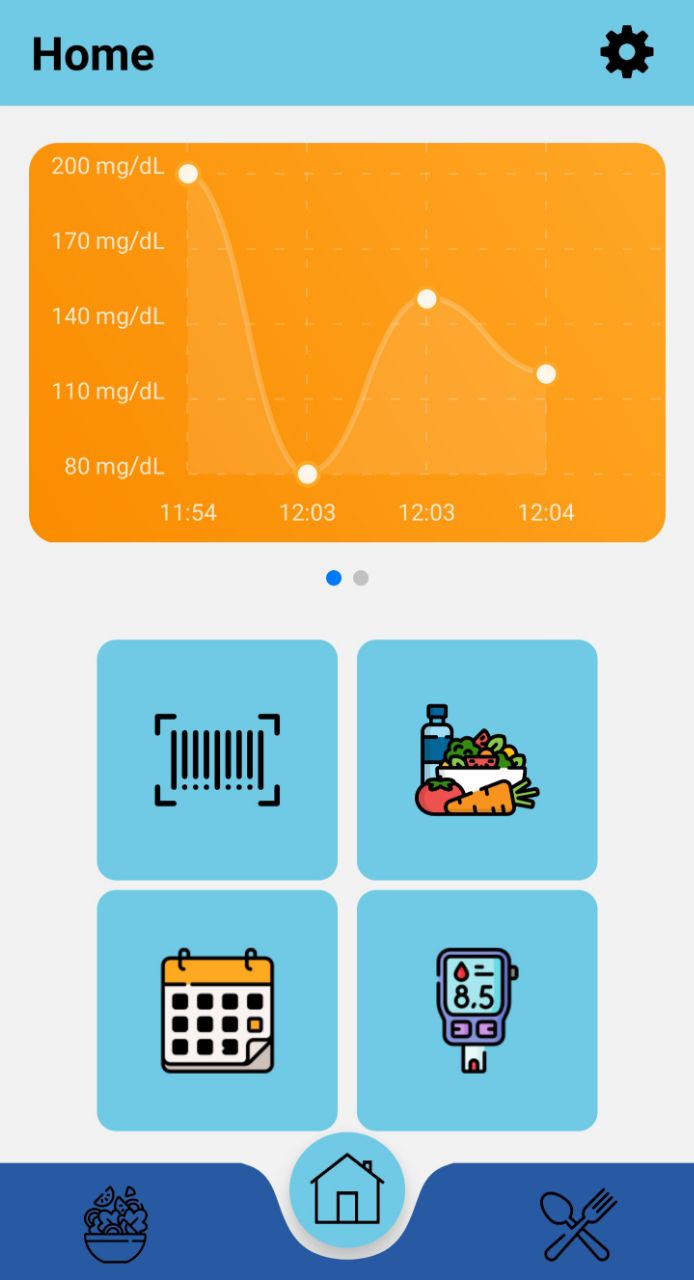
\includegraphics[scale=0.2]{screenshot3}
\end{center}

	\subsection{Search}
    Search food or recipe for nutritional details or to add it in meal diary. User can easly modify the unit measure and quantity of food.
	\begin{center}

		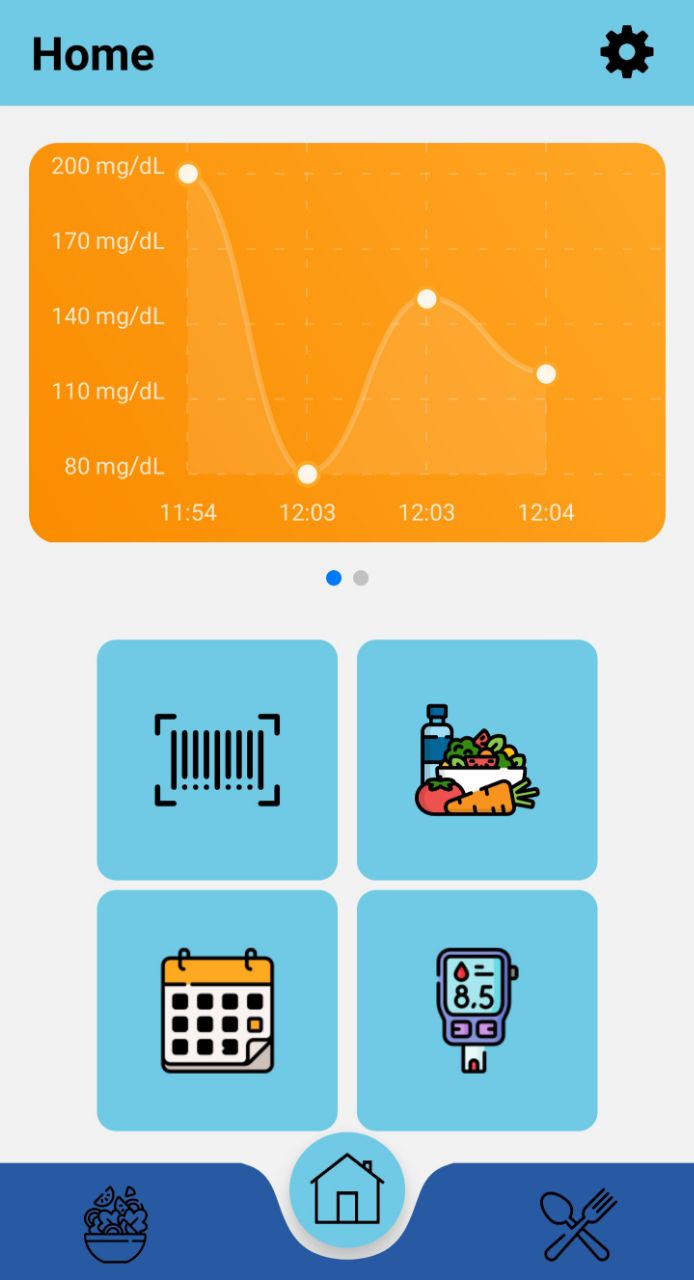
\includegraphics[scale=0.2]{screenshot3}
	\end{center}

	\subsection{Glycemia PopUp}
    Add glycemia quickly just using the menu shortcut or during the insulin caluclation procedure. The value 
	will automatically stored in Firebase.
	\begin{center}

		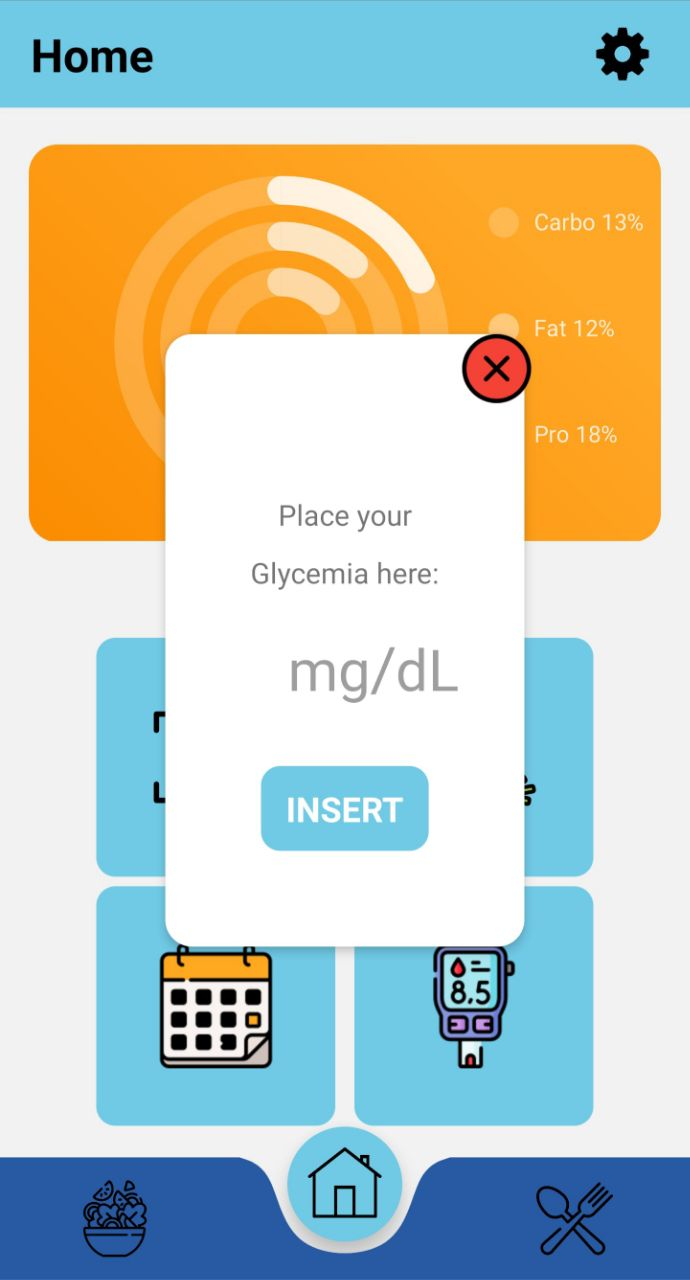
\includegraphics[scale=0.2]{screenshot1}
	\end{center}


	\subsection{Meal Diary}
    Meal Diary can be used for both calulating daily total macro nutrients and insuline dose of each meal. 
	\begin{center}

		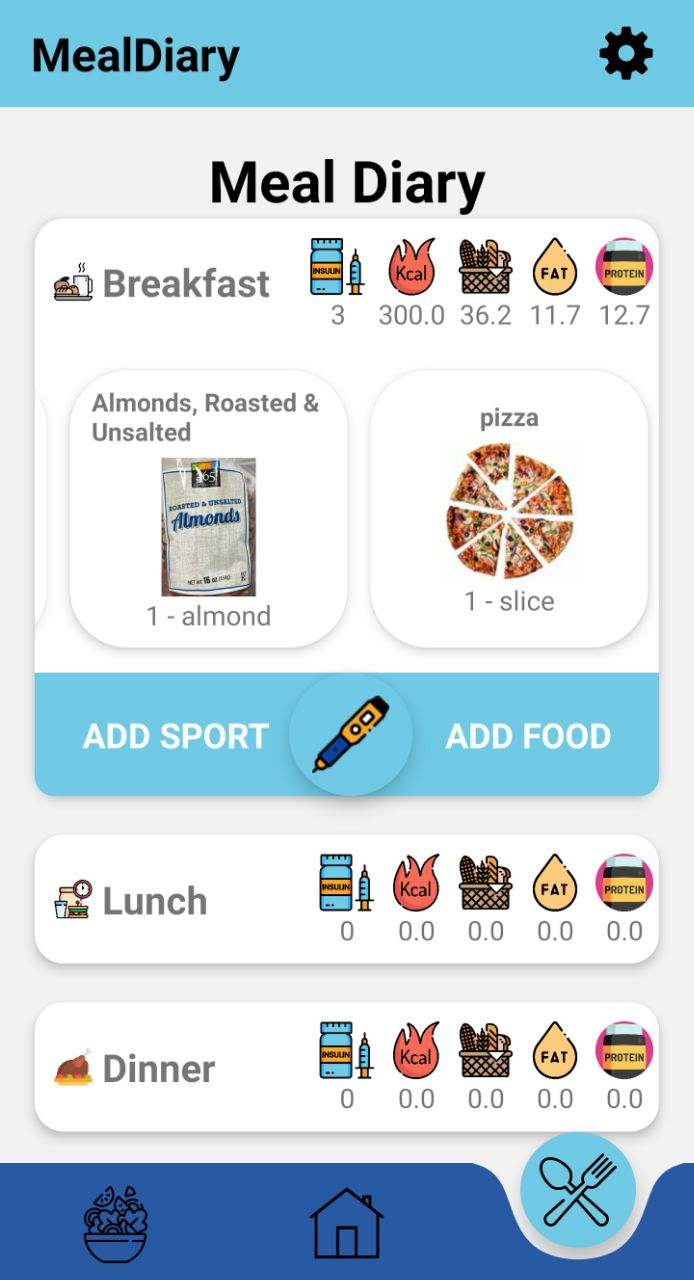
\includegraphics[scale=0.2]{screenshot5}
	\end{center}

	\subsection{Calendar}
	In calendar it will be possible to retrieve historical data by clicking on a date. 
	\begin{center}

	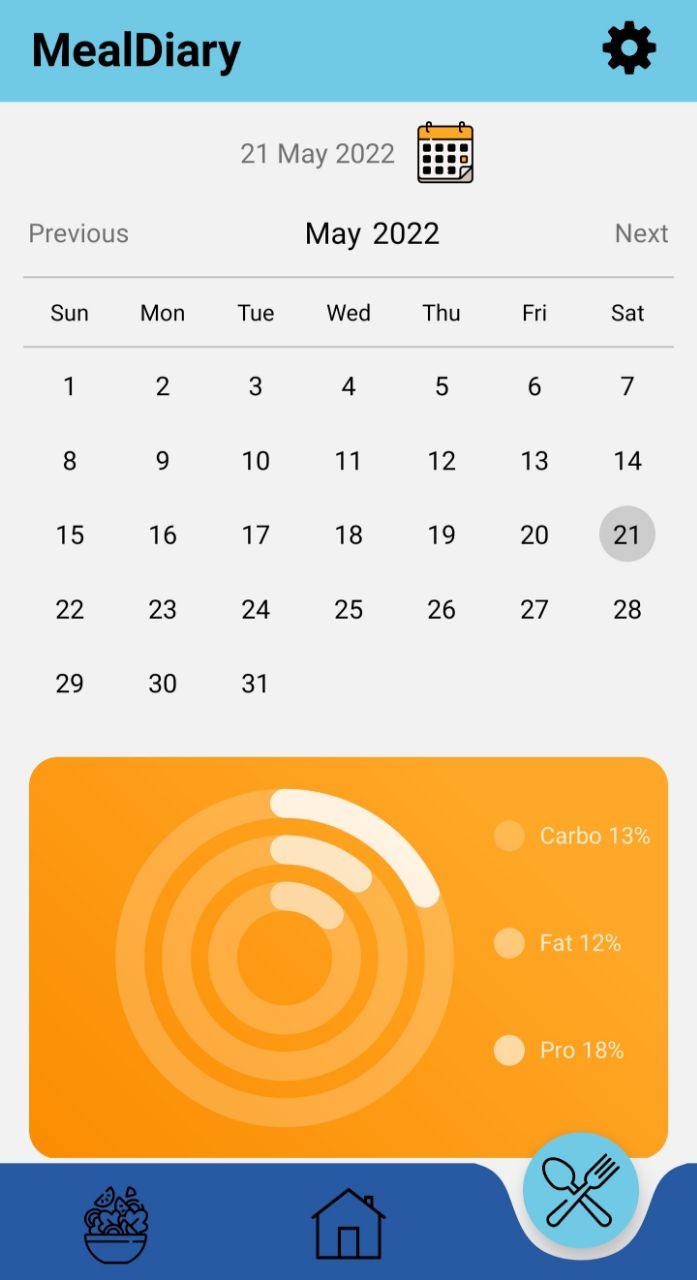
\includegraphics[scale=0.2]{screenshot4}
\end{center}

\newpage
%%%%%%%%%%%%%%%%%%%%%%%%%%%%%%%%%%%%%%%%%%%%%%%%%%%%%%%%%%%
\section{Architecture}
\vspace{10.5cm}
	The technology used to make this app is react native \cite{React Native}.
	
\includegraphics[scale=0.1]{RN}
	\subsection{Folder Structure}
	\begin{docCommand}{assets}{}
		Contains all images and component with a proper mapping.
	\end{docCommand}

	\begin{docCommand}{constants}{}
		All constants concerning the design and states of the app.
	\end{docCommand}

	\begin{docCommand}{customComponents}{}
		All buttons, charts and pickers specifically designed for the pages.
	\end{docCommand}

	\begin{docCommand}{pages}{}
		Folder with all pages of the app, using the custom components
	\end{docCommand}

	\begin{docCommand}{stateManager}{}
		Redux States for data managing with actions and reducers: macroTracker for meals and userReducer for the patient.
	\end{docCommand}

	\begin{docCommand}{utils}{}
		Logic of API, authentication, Firebase and Insulin Calculator
	\end{docCommand}




\newpage
%%%%%%%%%%%%%%%%%%%%%%%%%%%%%%%%%%%%%%%%%%%%%%%%%%%%%%%%%%%
\section{API doc}	
\vspace{10.5cm}	
	\subsection{Nutritionix}\label{subsec:mathenvironments}
		Nutritionix \cite{Nutritionix} is the API used to have a food database-
	\subsection{Firebase}
	    Firebase \cite{Firebase} is a Google serverless platorm for application development. 
		
\newpage
%%%%%%%%%%%%%%%%%%%%%%%%%%%%%%%%%%%%%%%%%%%%%%%%%%%%%%%%%%%
\section{Redux States}
\vspace{10.5cm}
	Inserting grap
%%%%%%%%%%%%%%%%%%%%%%%%%%%%%%%%%%%%%%%%%%%%%%%%%%%%%%%%%%%
\section{Insulin Calculator}
\vspace{10.5cm}
	Inserting graphics in your document requires the  \textbf{graphicx package}, which you can find in the folder that accompanied this guide.
	\subsection{Easiest Way to Insert Images}
	The easiest, most straightforward way I have found so far to insert images into your LaTeX document is through TeX Studios include graphics feature. This features allows you to bypass having to constantly type and communicate with your computer where the folder containing your images is located. This really comes in handy once one has created several latex documents across several folders. If you decide to insert images through this method, as I presume most of those reading this will, \textbf{make sure to remove the graphics path command from the preamble of the templates in the folder containing this pdf.}
\vspace{4mm}\\
	So to insert an image into your \LaTeX\ file, go to the taskbar located at the top of your screen and click the menu labeled \textbf{LaTeX}. Inside the LaTeX dropdown, go down to \textbf{Input/Include Files} and then \textbf{includegraphics}. Once there, find where you put the image you wanted to insert into your document and then press ok.
	\subsection{Graphics Path}
	Most of the time, it will easier to insert images into a file using the method we mentioned in the previous subsection. However, the following allows for a cleaner, more organized, but a little more complicated at times possibly more advanced way to insert images into your \LaTeX\ file.
		\begin{docCommand}{graphicspath}{\brackets{path}}
			This command prevents you from having to tell the computer where the image is stored each time you wanted to insert an image.\\
			The easiest way to set up the graphicspath is to create a folder where you store all the images you want to use and label it \textbf{images}. You put this folder in the same area where you write your files. Then you input the following at the beginning of your document: 
			\begin{verbatim}
				\graphicspath{{./images/}}
			\end{verbatim}
		\end{docCommand}
	\subsection{Inserting Images}
		Once you have set up the graphics path from above, you insert pictures by using the following command:
		\begin{docCommand}{includegraphics}{\brackets{\sl{file-name}}}
			This command allows you to actually insert the image in the document. To alter the position and size of the image, see~\url{https://www.overleaf.com/learn/latex/Inserting_Images}.\\
		\end{docCommand} \vspace{1mm}
		To change the scale of file, use the following
		\begin{verbatim}
			\includegraphics[scale= ]{image file name}
		\end{verbatim}
	\subsection{Image Additions}
		\begin{docCommand}{caption}{\brackets{\sl{text}}}
			Allows you to add a caption to an image.
		\end{docCommand}
		\begin{docEnvironment}{wrapfigure}{}
			Allows you to wrap an image inside text. For more on this, see the wrapfigure.pdf inside the wrapfigure folder.
		\end{docEnvironment}
	\subsection{Positioning an Image}
		To alter an images position: see \url{https://www.overleaf.com/learn/latex/Inserting_Images}
\newpage
\newgeometry{
	left=20mm, 
	right=20mm, 
	top=20mm, 
	bottom=20mm}
%%%%%%%%%%%%%%%%%%%%%%%%%%%%%%%%%%%%%%%%%%%%%%%%%%%%%%%%%%%
\section{Testing}
\vspace{10.5cm}

To perform automated and personalized testing it was used Jest \cite{Jest}. It is a JavaScript Testing Framework that supports React Native.
Tests were performed on:
\begin{docCommand}{__tests__}{}
Where to overcome some technological barriers, mock objects were used instead of not supported libraries.
\end{docCommand}

\subsection{Folders}


\begin{docCommand}{api-test}{}
	Local storage and API calls from Firebase and Nutritionix.
\end{docCommand}

\begin{docCommand}{redux-test}{}
	Redux and user actions such as: adding food to meal or removing it. 
\end{docCommand}

\begin{docCommand}{renders-test}{}
	Checks correct Pages rendering. Makes snapshots of all pages and compares them with expected result.
\end{docCommand}

\begin{docCommand}{utils}{}
   Checks User input and Insulin Calculator 
\end{docCommand}


\newpage
\newgeometry{
	left=32mm, right=18mm, top=20mm, bottom=18mm,
	marginparwidth=28mm, marginparsep=4mm}
%%%%%%%%%%%%%%%%%%%%%%%%%%%%%%%%%%%%%%%%%%%%%%%%%%%%%%%%%%%
\section{Future Implementations}
\vspace{10.5cm}
----
\newpage
%%%%%%%%%%%%%%%%%%%%%%%%%%%%%%%%%%%%%%%%%%%%%%%%%%%%%%%%%%%
\section{Future Implementations}
\begin{thebibliography}{17}
	\vspace{10.5cm}
		\bibitem{Type 1 Diabetes} Diabetes Definition\\
				\url{https://en.wikipedia.org/wiki/Type_1_diabetes}
		\bibitem{Bolus} Bolus Definition\\
				\url{https://en.wikipedia.org/wiki/Bolus_(medicine)}
		\bibitem{React Native} React Native\\
				\url{https://reactnative.dev}
		\bibitem{Nutritionix} Nutritionix\\
				\url{https://www.nutritionix.com}
		\bibitem{Jest} Jest\\
				\url{https://jestjs.io}
		\bibitem{Firebase} Firebase\\
				\url{https://firebase.google.com}
	\end{thebibliography}
\addtocounter{section}{14}
\addcontentsline{toc}{section}{\protect\numberline{\thesection}~~~ References}
%%%%%%%%%%%%%%%%%%%%%%%%%%%%%%%%%%%%%%%%%%%%%%%%%%%%%%%%%%%%%%%%%%
\end{document}